\section{Contexte et définition du problème}


\subsection{Danger des batteries Li-Ion}
% merger avec la version à l'école

\subsection{Système de protection et de gestion de batterie}

cellule, module, batterie, BMS, BPS

\subsection{Projet spécial}

École de technologie supérieur

\subsection{Club étudiant Éclipse}

\paragraph{}
Éclipse est un club étudiant composé d'une quarantaine d'étudiants en ingénierie qui ont pour objectif de construire une véhicule alimenter par l'énergie solaire à l'aide de panneaux photovoltaïques. Depuis sa fondation en 1992, neuf prototypes ont été construit en y intégrant les technologies de pointes disponibles au moment de leurs conceptions. Similaire aux voitures électriques, le véhicule solaire possède une chaîne de traction électrique comme moyen de propulsion. Les moteurs roues  CSIRO sont alimentés par des entraînement électrique qui sont à leur tour alimentés bar une batterie. Depuis quelques années, l'équipe s'est tourné vers l'utilisation d'accumulateurs au Li-ion. Il est donc nécessaire d'avoir un système de protection et de gestion de batterie.

\paragraph{}
Une des philosophies du club est de concevoir par les étudiants le plus de modules possible. Le temps de développement du dernier système de protection et de gestion de batterie à pris environ 7 ans et comme la conception d'un nouveau véhicule se fait à tous les deux ans, la disposition des batteries changent beaucoup. C'est pourquoi les deux derniers prototypes ont utilisés des systèmes acheter par manque de temps. L'intégration de système provenant de compagnie accélère le temps de fabrications du véhicule mais ne permet pas le contrôle total du système et l'expertise de conception de ces systèmes se perd au sein du club puisqu'il y a un gros roulement des étudiants. Il faut également des systèmes fiables et robustes, ce qui peut être difficile à concevoir lorsque ce système est aussi critique qu'un système de protection et de gestion de batterie. Une défaillance de ce système pourrait mener la destruction partiel ou total du véhicule et la vie du pilote est en jeu. D'autant plus que le véhicule solaire sera soumis à plusieurs épreuves dans des conditions de route réelles et en circuit fermé durant les compétitions.

\subsection{Compétitions}


\subsubsection{ASC2016}

Scruteneering

\subsubsection{Compétitions futures}

Règlements


FSGP2017
ASC2018
WSC2019



\subsection{Rétrocompatibilité}



BMS Lithium Balance

%\begin{figure}[h!]
%	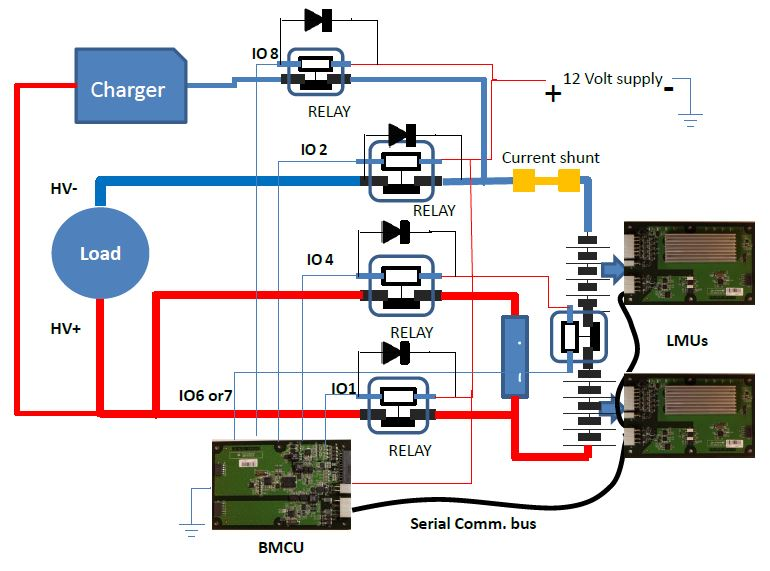
\includegraphics[width=\linewidth]{Hardware.jpg}
%	\caption{Disposition matériel du système de protection}
%	\label{fig:Disposition matériel}
%\end{figure}
%
%Pin out
%
%\begin{figure}[h!]
%	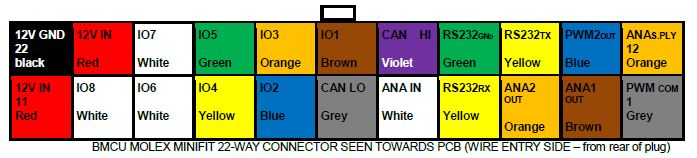
\includegraphics[width=\linewidth]{Pinout.jpg}
%	\caption{Brochage du connecteur}
%	\label{fig:Brochage1}
%\end{figure}
%
%\begin{figure}[h!]
%	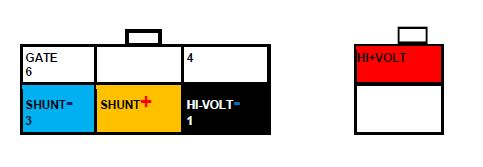
\includegraphics[width=\linewidth]{Pinout2.jpg}
%	\caption{Brochage du connecteur}
%	\label{fig:Brochage2}
%\end{figure}
%
%Fonctions